\documentclass[c]{beamer}

\usepackage[utf8]{inputenc}
\usepackage{lmodern} 
%\usepackage[scaled=0.8]{beramono}
\usepackage[T1]{fontenc}
\usepackage{microtype}

\usepackage{graphicx}
\usepackage{float}
\usepackage[hypcap]{caption}
\usepackage{subcaption}
\usepackage{algorithm2e}
\usepackage{array}

\usepackage{media9}

\usepackage{mathtools}
\usepackage{amssymb}
\usepackage{amsthm}
\usepackage{amsmath}


\usepackage[utf8]{inputenc}
\usepackage{lmodern} 
%\usepackage[scaled=0.8]{beramono}
\usepackage[T1]{fontenc}
\usepackage{microtype}

\usepackage{graphicx}
\usepackage{float}
\usepackage[hypcap]{caption}
\usepackage{subcaption}
\usepackage{algorithm2e}
\usepackage{array}

\usepackage{media9}

\usepackage{amssymb}
\usepackage{amsthm}
\usepackage{amsmath}


\usepackage{mathtools}

%\usepackage[customcolors]{hf-tikz}
%\usepackage{pgfplots}



%\usepackage{animate}
%\usepackage{movie15}

%\usepackage{epstopdf}

%\epstopdfDeclareGraphicsRule{.gif}{png}{.png}{convert gif:#1 png:\OutputFile}
%\AppendGraphicsExtensions{.gif}



\usepackage[english]{babel}
\selectlanguage{english}

\usetheme{Warsaw}
%\usetheme{CambridgeUS}
\usecolortheme{crane}
\beamertemplatenavigationsymbolsempty

\newcommand{\inred}[1]{\textcolor{red}{#1}}
\newcommand{\inblue}[1]{\textcolor{blue}{#1}}

\beamertemplatenavigationsymbolsempty
\setbeamertemplate{footline}[page number]{}

\captionsetup[figure]{labelformat=empty}


\newcommand{\Prod}[2]{(#1, #2)_{L^2}}
\newcommand{\Mat}[1]{\mathbf{#1}}

\newcommand{\dx}{\, \mathrm{d}x}
\newcommand{\deriv}[2]{\frac{\partial {#1}}{\partial {#2}}}
\newcommand{\Int}[1]{\int_0^1 {#1}\dx}
\newcommand{\Lims}[1]{\left. #1 \right|_0^1}
\newcommand{\IntE}[2]{\int_{#1}{#2}\dx}
\newcommand{\der}[1]{{#1}^\prime}
\newcommand{\Vect}[1]{\mathbf{#1}}

\newcommand{\A}[1]{\Mat{A}\big(#1\big)}
\newcommand{\Bsp}{\mathcal{B}}
\newcommand{\E}[1]{\left[\xi_{#1}, \xi_{#1 + 1}\right]}
\newcommand{\Different}[1]{\textcolor{blue}{#1}}



\title{%
Scaling Out Alternating Direction Isogeometric L2 Projections Solver}

\author{%
    \inblue{\bf Grzegorz Gurgul (AGH)} \\
        \inblue{Bartosz~Bali\'{s} (AGH)} \\
    \inblue{Marcin \L{}o\'{s} (AGH)} \\
    \inblue{Danuta~Szeliga (AGH)} \\
      \inblue{Maciej Paszy\'{n}ski (AGH)} }
\date{{\bf 14th U.S. National Congress on Computational Mechanics} \break \break July 17-20, 2017, Montreal, Canada}

\begin{document}

%%%%%%%%%%%%%%%%%%%%%%%%%%%

\begin{frame}
  \titlepage
\end{frame}

%%%%%%%%%%%%%%%%%%%%%%%%%%%
\begin{frame}{Agenda}

\begin{itemize}
  \item Background
  \item Isogeometric L2 projections solver - theory
  \item Isogeometric L2 projections solver - algorithm
  \item Isogeometric L2 projections solver - implementation
  \item Conclusions
\end{itemize}

\end{frame}

%%%%%%%%%%%%%%%%%%%%%%%%%%%

\begin{frame}{Background}

{\small
\begin{itemize}
  \item Isogeometric L2 projections algorithm
\end{itemize}
  \inblue{Proposed by prof. Victor Calo:} 
L. Gao, V.M. Calo, \it{Fast Isogeometric Solvers for Explicit Dynamics}, {\bf Computer Methods in Applied Mechanics and Engineering} (2014). 
\begin{itemize}
  \item Applications to time-dependent problems
\end{itemize}
\inblue{Non-linear flow (Fortran+MPI, parallel ): }
M. Wo\'{z}niak, M. \L{}o\'{s}, M. Paszy\'{n}ski, L. Dalcin, V. Calo, 
\it{Parallel fast isogeometric solvers for explicit dynamics}, {\bf Computing and Informatics} (2015)
\vspace{2mm}

\inblue{Tumor growth simulations (C++ sequential ): }M. \L{}o\'{s}, M. Paszy\'{n}ski, A. K\l{}usek, W. Dzwinel, \it{Application of fast isogeometric L2 projection solver for tumor simulations}, {\bf Computer Methods in Applied Mechanics and Engineering} (2017)  
}

\end{frame}


%%%%%%%%%%%%%%%%%%%%%%%%%%%%%%%%%%%%%%%

%%%%%%%%%%%%%%%%%%%%%%%%%%%

\begin{frame}{Background}

\begin{itemize}
  \item Improving performance of time-dependent applications of ADS
\end{itemize}

\inblue{Step 1: CUDA implementation: }\break
G. Gurgul, M. Paszy\'{n}ski, D. Szeliga, 
\it{Open source JAVA implementation of the parallel multi-thread alternating direction isogeometric L2 projections solver for material science simulations}, {\bf USACM Conference on Isogeometric Analysis and Meshfree Methods} (2016) 

\vspace{1mm}
\inblue{Step 2: Object-Oriented shared memory implementation: }\break
G. Gurgul, M. Paszy\'{n}ski, D. Szeliga, 
\it{Open source JAVA implementation of the parallel multi-thread alternating direction isogeometric L2 projections solver for material science simulations}, {\bf Computer Methods in Material Science} (2017) 

\vspace{1mm}
\inred{\bf Step 3: Cloud implementation: }\break
G. Gurgul, Bartosz~Bali\'{s},  Marcin \L{}o\'{s}, D. Szeliga, M. Paszy\'{n}ski, \it{Scaling Out Alternating Direction Isogeometric L2 Projections Solver}, {\bf 14th U.S. National Congress on Computational Mechanics}


\end{frame}




%%%%%%%%%%%%%%%%%%%%%%%%%%%%%%%%%%%%%%%

% INTRO
%%%%%%%%%%%%%%%%%%%%%%%%%%%

\begin{frame}{Isogeometric $L^2$ projections}


\textbf{In general:} non-stationary problem of the form

\begin{equation*}
  \partial_t u - \mathcal{L}(u) = f(x, t) \implies  \sum_{ij} u_{ij} \Prod{B_{ij}}{B_{kl}} = RHS
\end{equation*}

with some initial state~$u_0$ and boundary conditions
\vspace{2mm}

$\mathcal{L}$ -- well-posed linear spatial partial differential operator

\vspace{3mm}

Discretization:
\begin{itemize}
  \item spatial discretization: isogeometric FEM
  \\\vspace{2mm}
  Basis functions: $\phi_1,\ldots,\phi_n$ (tensor product B-splines)
  \\\vspace{2mm}
  \item time discretization with explicit method
  \\\vspace{2mm}
  \item implies isogeometric $L^2$ projections in every time step 
  
\end{itemize}

\end{frame}


%%%%%%%%%%%%%%%%%%%%%%%%%%%

\begin{frame}{$L^2$ projections -- tensor product basis}

\begin{figure}
  \centering
  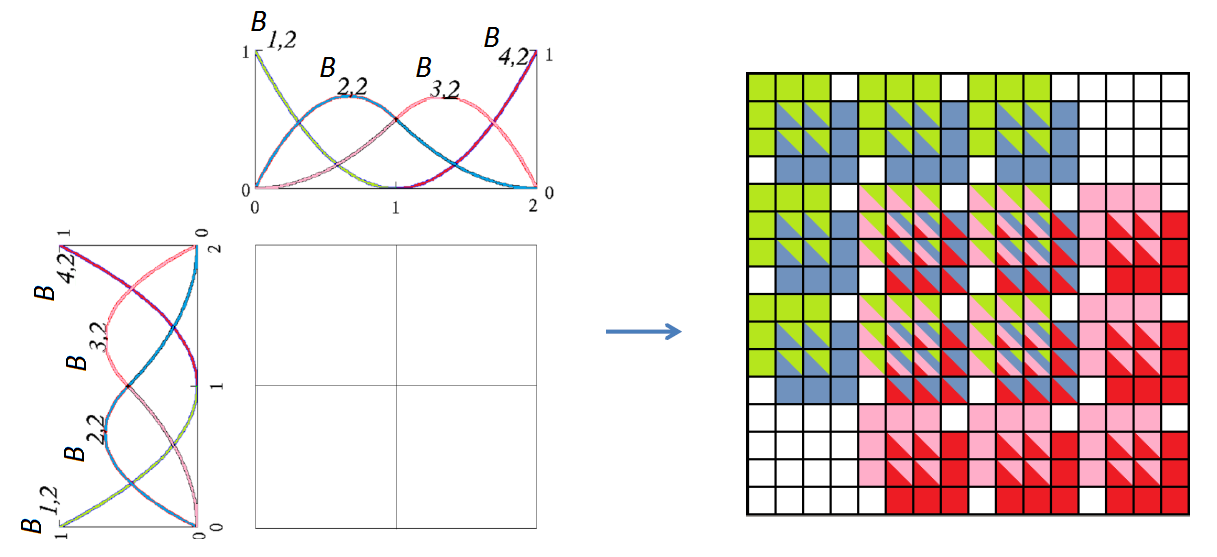
\includegraphics[width=0.8\textwidth]{img/2DFEM}
\end{figure}

Isogeometric basis functions:
\begin{itemize}
  \item 1D B-splines basis $B_1(x),\ldots, B_n(x)$
  \item higher dimensions: tensor product basis\\
        $B_{i_1\cdots i_d}(x_1,\ldots,x_d)
        \equiv B^{x_1}_{i_1}(x_1)\cdots B^{x_d}_{i_d}(x_d)$ \\
\end{itemize}
Gram matrix of B-spline basis on 2D domain $\Omega = \Omega_x \times \Omega_y$:

\begin{equation*}
  \begin{aligned}
  \mathcal{M}_{ijkl} &=
  \Prod{B_{ij}}{B_{kl}} =
  \int_\Omega B_{ij}B_{kl}\,\mbox{d}\Omega 
  \end{aligned}
\end{equation*}

\end{frame}

%%%%%%%%%%%%%%%%%%%%%%%%%%%

\begin{frame}{$L^2$ projections -- tensor product basis}

Isogeometric basis functions:
\begin{itemize}
  \item 1D B-splines basis $B_1(x),\ldots, B_n(x)$
  \item higher dimensions: tensor product basis\\
        $B_{i_1\cdots i_d}(x_1,\ldots,x_d)
        \equiv B^{x_1}_{i_1}(x_1)\cdots B^{x_d}_{i_d}(x_d)$ \\
\end{itemize}
Gram matrix of B-spline basis on 2D domain $\Omega = \Omega_x \times \Omega_y$:
\begin{equation*}
  \begin{aligned}
  \mathcal{M}_{ijkl} &=
  \Prod{B_{ij}}{B_{kl}} =
  \int_\Omega B_{ij}B_{kl}\,\mbox{d}\Omega 
  \end{aligned}
\end{equation*}
 \inblue{\begin{equation*}
  \begin{aligned}
=\int_\Omega B^x_i(x) B^y_j(y) B^x_k(x) B^y_l(y) \,\mbox{d}\Omega \\
  = \int_\Omega (B_i B_k)(x)\,(B_j B_l)(y)\,\mbox{d}\Omega  \\
  = \left(\int_{\Omega_x} B_i B_k \,\mbox{d}x\right)
  \left(\int_{\Omega_y} B_j B_l \,\mbox{d}y\right) \\
  = \mathcal{M}^x_{ik} \mathcal{M}^y_{jl}
  \end{aligned}
\end{equation*}}
\begin{equation*}
\mathcal{M} = \mathcal{M}^x \otimes \mathcal{M}^y \quad\text{(Kronecker product)}
\end{equation*}

\end{frame}

%%%%%%%%%%%%%%%%%%%%%%%%%%%

\begin{frame}{Gram matrix of tensor product basis}

\begin{figure}
  \centering
  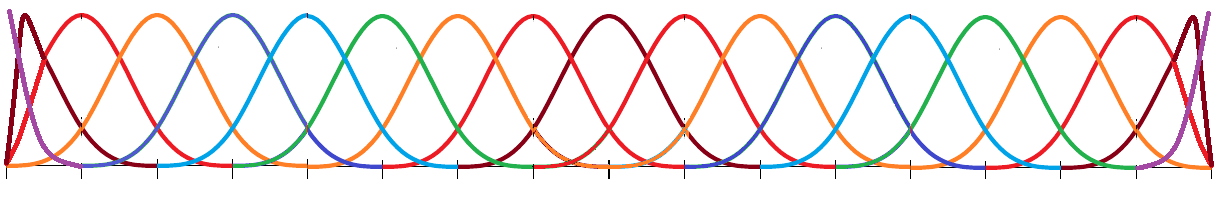
\includegraphics[width=0.6\textwidth]{img/Bsplines}
\end{figure}

B-spline basis functions have \textbf{local support} (over $p+1$ elements) 

$\mathcal{M}^x$, $\mathcal{M}^y$, \ldots -- banded structure

$\mathcal{M}^x_{ij} = 0 \iff |i - j| > 2p + 1$

Exemplary basis functions and matrix for cubics

\begin{tiny}
\begin{equation*}
	\begin{bmatrix}
    \Prod{B_1}{B_1} & \Prod{B_1}{B_2} & \Prod{B_1}{B_3} & \Prod{B_1}{B_4} & 0 & 0 & \cdots & 0 \\
    \Prod{B_2}{B_1} & \Prod{B_2}{B_2} & \Prod{B_2}{B_3} & \Prod{B_2}{B_4} & \Prod{B_2}{B_5} & 0 & \cdots & 0 \\
    \Prod{B_3}{B_1} & \Prod{B_3}{B_2} & \Prod{B_3}{B_3} & \Prod{B_3}{B_4} & \Prod{B_3}{B_5} & \Prod{B_3}{B_6} & \cdots & 0 \\
    \vdots & \vdots & \vdots & \vdots &  \vdots & \vdots &  & \vdots\\
    0 & 0 & \ldots & \Prod{B_n}{B_{n-3}}& \Prod{B_n}{B_{n-2}} & \Prod{B_n}{B_{n-1}} & \Prod{B_n}{B_n}
  \end{bmatrix}
\end{equation*}
\end{tiny}

\end{frame}


%%%%%%%%%%%%%%%%%%%%%%%%%%%

\begin{frame}[fragile]{Alternating Direction Solver -- 2D}

{Two steps} -- solving systems with $\Mat{A}$ and $\Mat{B}$ in different \emph{directions}
\begin{equation*}
  \begin{bmatrix}
    A_{11} & A_{12} & \cdots & 0 \\
    A_{21} & A_{22} & \cdots & 0 \\
    \vdots & \vdots & \ddots & \vdots \\
    0 & 0 & \cdots & A_{nn} \\
  \end{bmatrix}
  \begin{bmatrix}
    y_{11} & y_{21} & \cdots & y_{m1}
    \\
    y_{12} & y_{22} & \cdots & y_{m1}
    \\
    \vdots & \vdots & \ddots & \vdots \\
    y_{1n} & y_{2n} & \cdots & y_{mn}
    \\
  \end{bmatrix}
  =
  \begin{bmatrix}
    b_{11} & b_{21} & \cdots & b_{m1} \\
    b_{12} & b_{22} & \cdots & b_{m2} \\
    \vdots & \vdots & \ddots & \vdots \\
    b_{1n} & b_{2n} & \cdots & b_{mn} \\
  \end{bmatrix}
\end{equation*}
\begin{equation*}
  \begin{bmatrix}
    B_{11} & B_{12} & \cdots & 0 \\
    B_{21} & B_{22} & \cdots & 0 \\
    \vdots & \vdots & \ddots & \vdots \\
    0 & 0 & \cdots & B_{mm} \\
  \end{bmatrix}
  \begin{bmatrix}
    x_{11} & \cdots & x_{1n} \\
    x_{21} & \cdots & x_{2n} \\
    \vdots & \ddots & \vdots \\
    x_{m1} & \cdots & x_{mn} \\
  \end{bmatrix}
  =
  \begin{bmatrix}
    y_{11} &
    y_{12} & \cdots &
    y_{1n} \\
    y_{21} & y_{22} & \cdots & y_{2n} \\
    \vdots & \vdots & \ddots & \vdots \\
    y_{m1} &
    y_{m2} & \cdots &
    y_{mn} \\
  \end{bmatrix}
\end{equation*}

%$\Mat{A}$, $\Mat{B}$ -- multidiagonal matrices for one-dimensional bases \\
Two one dimensional problems with multiple RHS:
\begin{itemize}
\item $ n \times n $ with $m$ right hand sides $\rightarrow$ $O(n*m)=O(N)$
\item $ m \times m $ with $n$ right hand sides $\rightarrow$ $O(m*n)=O(N)$
\end{itemize}
\vspace{2mm}
Linear computational cost $O(N)$ as opposed to $O(N^{1.5})$ or $O(N^{2})$

\end{frame}



% MAIN PART
%%%%%%%%%%%%%%%%%%%%%%%%%%%

\begin{frame}{Algorithm - data structure}

The backing data structure is a tree. Each of its nodes holds coefficients of a simple linear equation being a portion of the original system.

\begin{columns}
  \begin{column}{0.2\textwidth}
  \begin{figure}
      \centering
      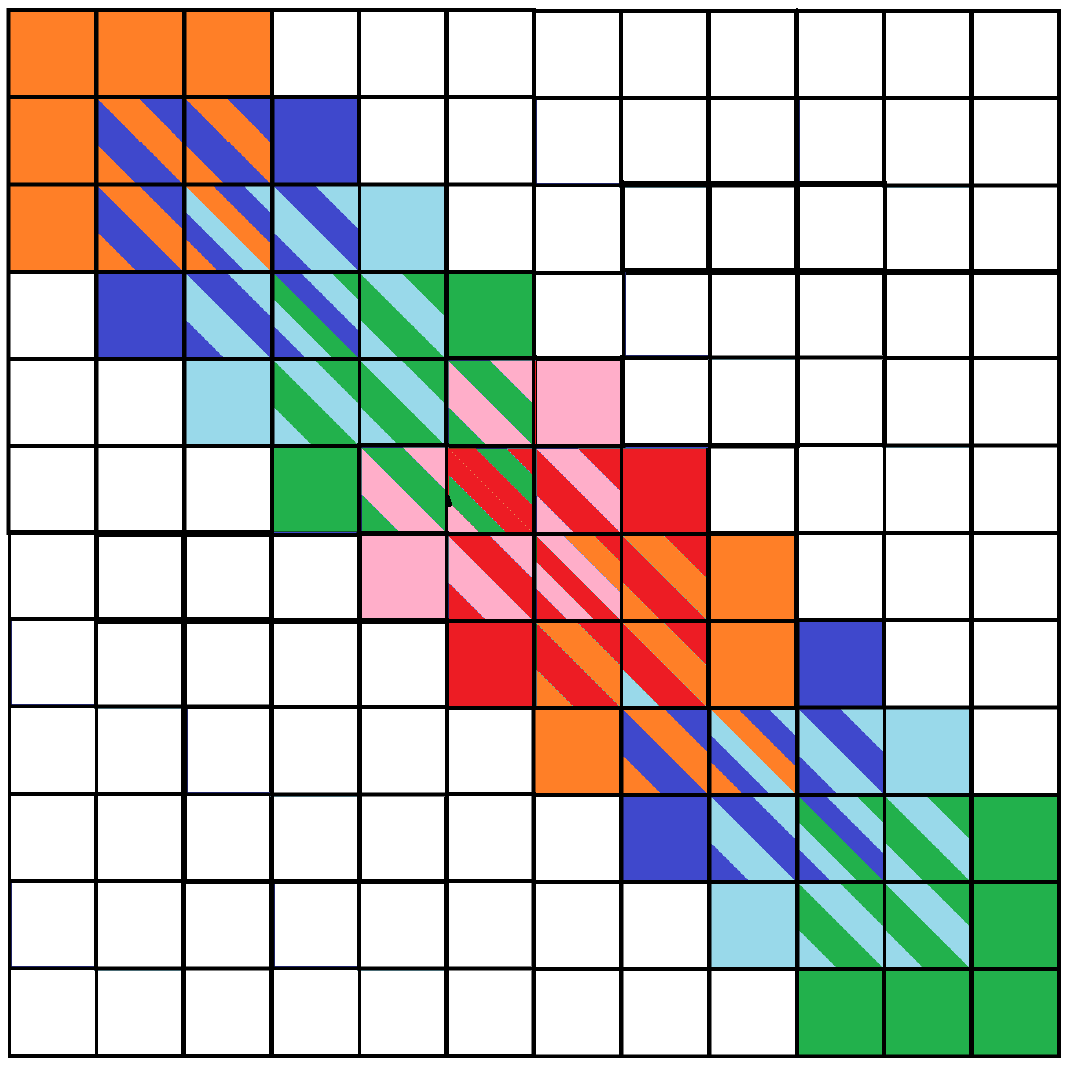
\includegraphics[width=1.1\textwidth]{img/partition}
      \caption{Partition of the problem matrix into sub-matrices}
    \end{figure}
  \end{column}

  \begin{column}{0.8\textwidth}
    \begin{figure}
      \centering
      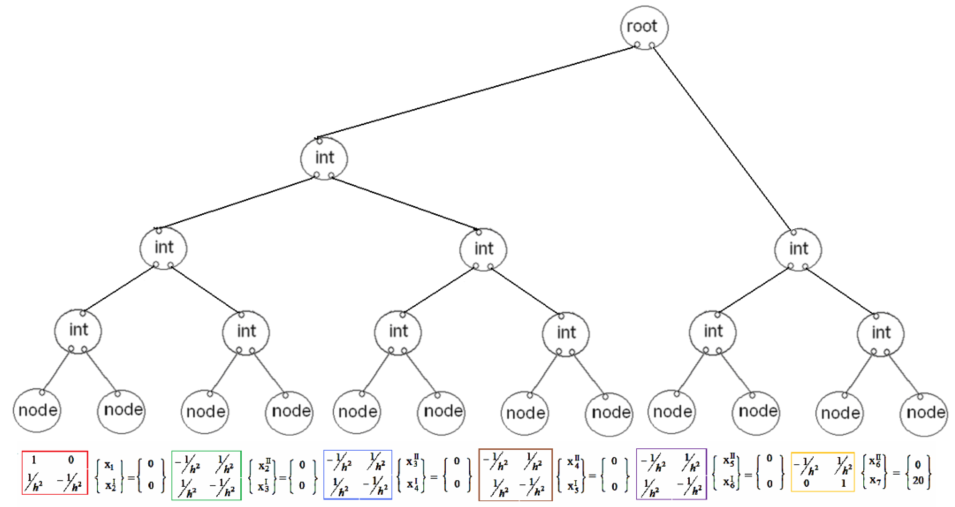
\includegraphics[width=0.95\textwidth]{img/tree_mat}
      \caption{Graph of matrices the solver will operate on}
    \end{figure}
  \end{column}
\end{columns}

\end{frame}


%%%%%%%%%%%%%%%%%%%%%%%%%%%

\begin{frame}{Algorithm - set of operations}

We can identify a set of basic tasks applicable on any vertex. We call them \textbf{productions}. They can:
\begin{itemize}
  \item branch a vertex into two \{$P1$, $P2$\} or three \{$P3$\} child vertices
  \item initialize a vertex with particular coefficients \{$A1$, $A$, $AN$\}
  \item merge two vertices and eliminate unknowns -  \{$A2\_3$, $E1\_2\_5$, $A2\_2$, $E2\_2\_6$, $Aroot$, $Eroot$\} 
  \item backward substitute parts of solution - \{$BS\_2\_6$, $BS\_1\_5$\}
\end{itemize}

\end{frame}

%%%%%%%%%%%%%%%%%%%%%%%%%%%

\begin{frame}{Algorithm - flow}

To obtain a solution for a 1-dimensional problem with 12 elements it is enough to execute the following productions, set by set, going from left to right, on respective vertices.

	\begin{figure}
      \centering
      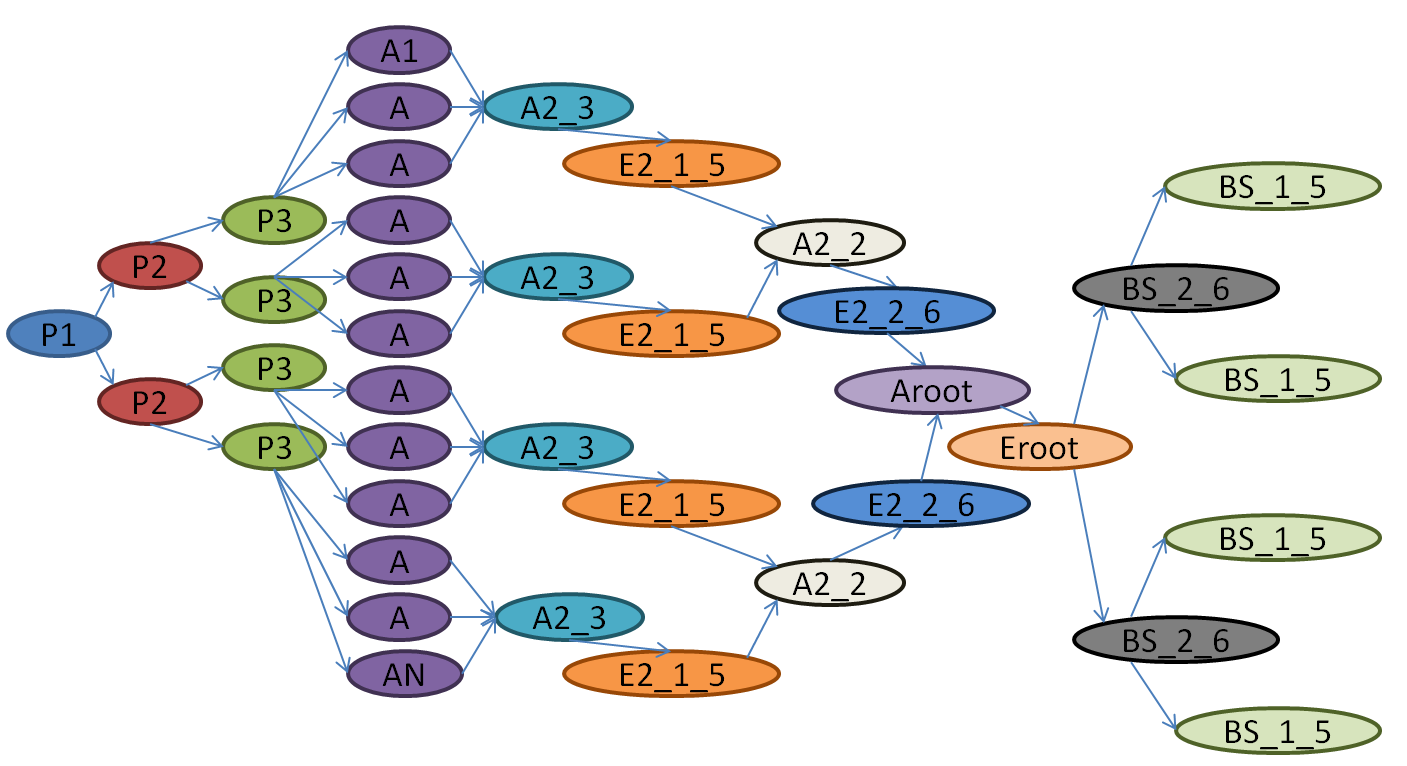
\includegraphics[width=1\textwidth]{img/task_tree}
    \end{figure}

\end{frame}

%%%%%%%%%%%%%%%%%%%%%%%%%%%

\begin{frame}{Implementation}

CUDA (GPU):
\begin{itemize}
  \item extremely fast for problems which \emph{fit in on-board memory}
  \item verbose and fragile
  \item hardware dependent
\end{itemize}

\vskip 0.1in

Shared memory (Multicore CPU)
\begin{itemize}
  \item fast for problems which fit in RAM ($37$ million elements require 16GB of RAM)
  \item portable, easy to understand and adapt
  \item scales up only
\end{itemize}

\vskip 0.1in

In memory grid (Cloud)
\begin{itemize}
  \item can solve problems of any size
  \item slower for relatively small problems
  \item \emph{scales out}
\end{itemize}

\end{frame}

%%%%%%%%%%%%%%%%%%%%%%%%%%%

\begin{frame}{Implementation - performance considerations}

Distributed environment implies \emph{heavy network traffic} and increased memory consumption due to \emph{extensive serialization}. This has to be reduced to the absolute minimum to let solver run bigger problems.
\vskip 0.1in

The following measures have been used:
\begin{itemize}
  \item split tree into set of subtrees of a given height and store them on a single node
  \item use localized map-reduce to extract columns from the solution rows
  \item reuse same operation on multiple vertices
  \item run subsequent operations applied on same vertex in one invocation
  \item schedule tasks in batches
  \item use near-caches
  \item keep solution in deserialized form
\end{itemize}

\end{frame}

%%%%%%%%%%%%%%%%%%%%%%%%%%%

\begin{frame}{Implementation - partition tree}

   \begin{figure}
      \centering
      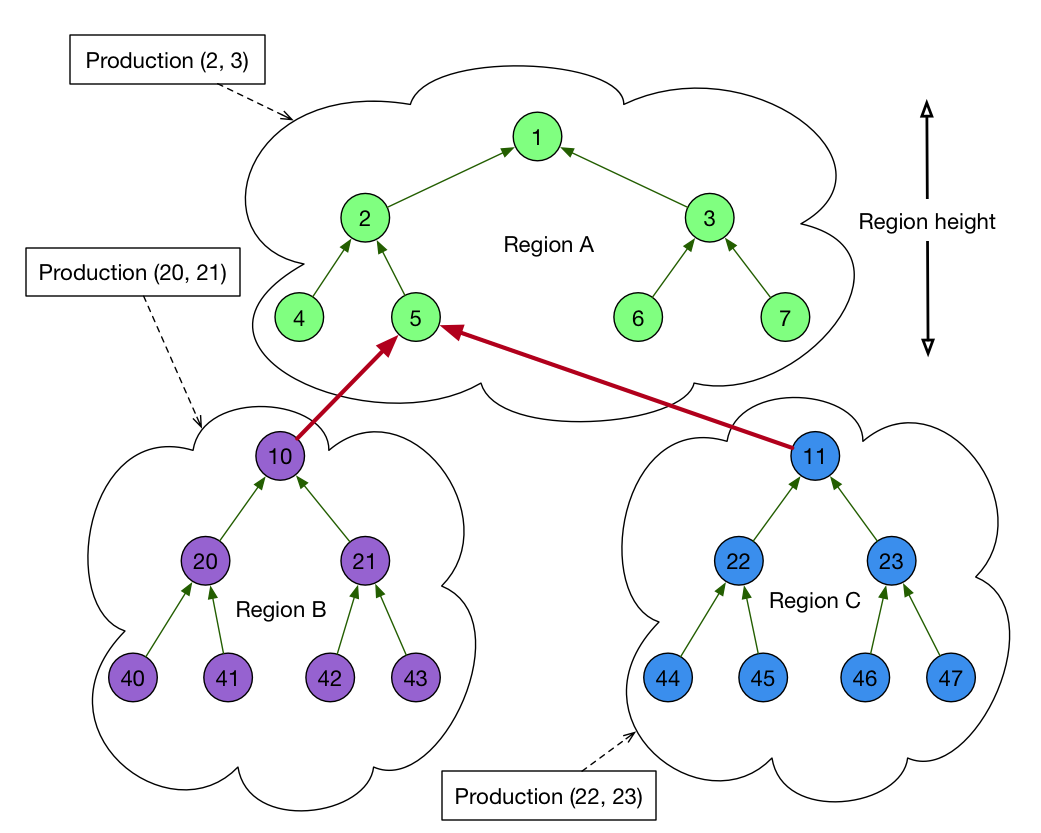
\includegraphics[width=0.9\textwidth]{img/graph-idea.png}
    \end{figure}

\end{frame}

%%%%%%%%%%%%%%%%%%%%%%%%%%%

\begin{frame}{Implementation - performance}

\begin{figure}
      \centering
      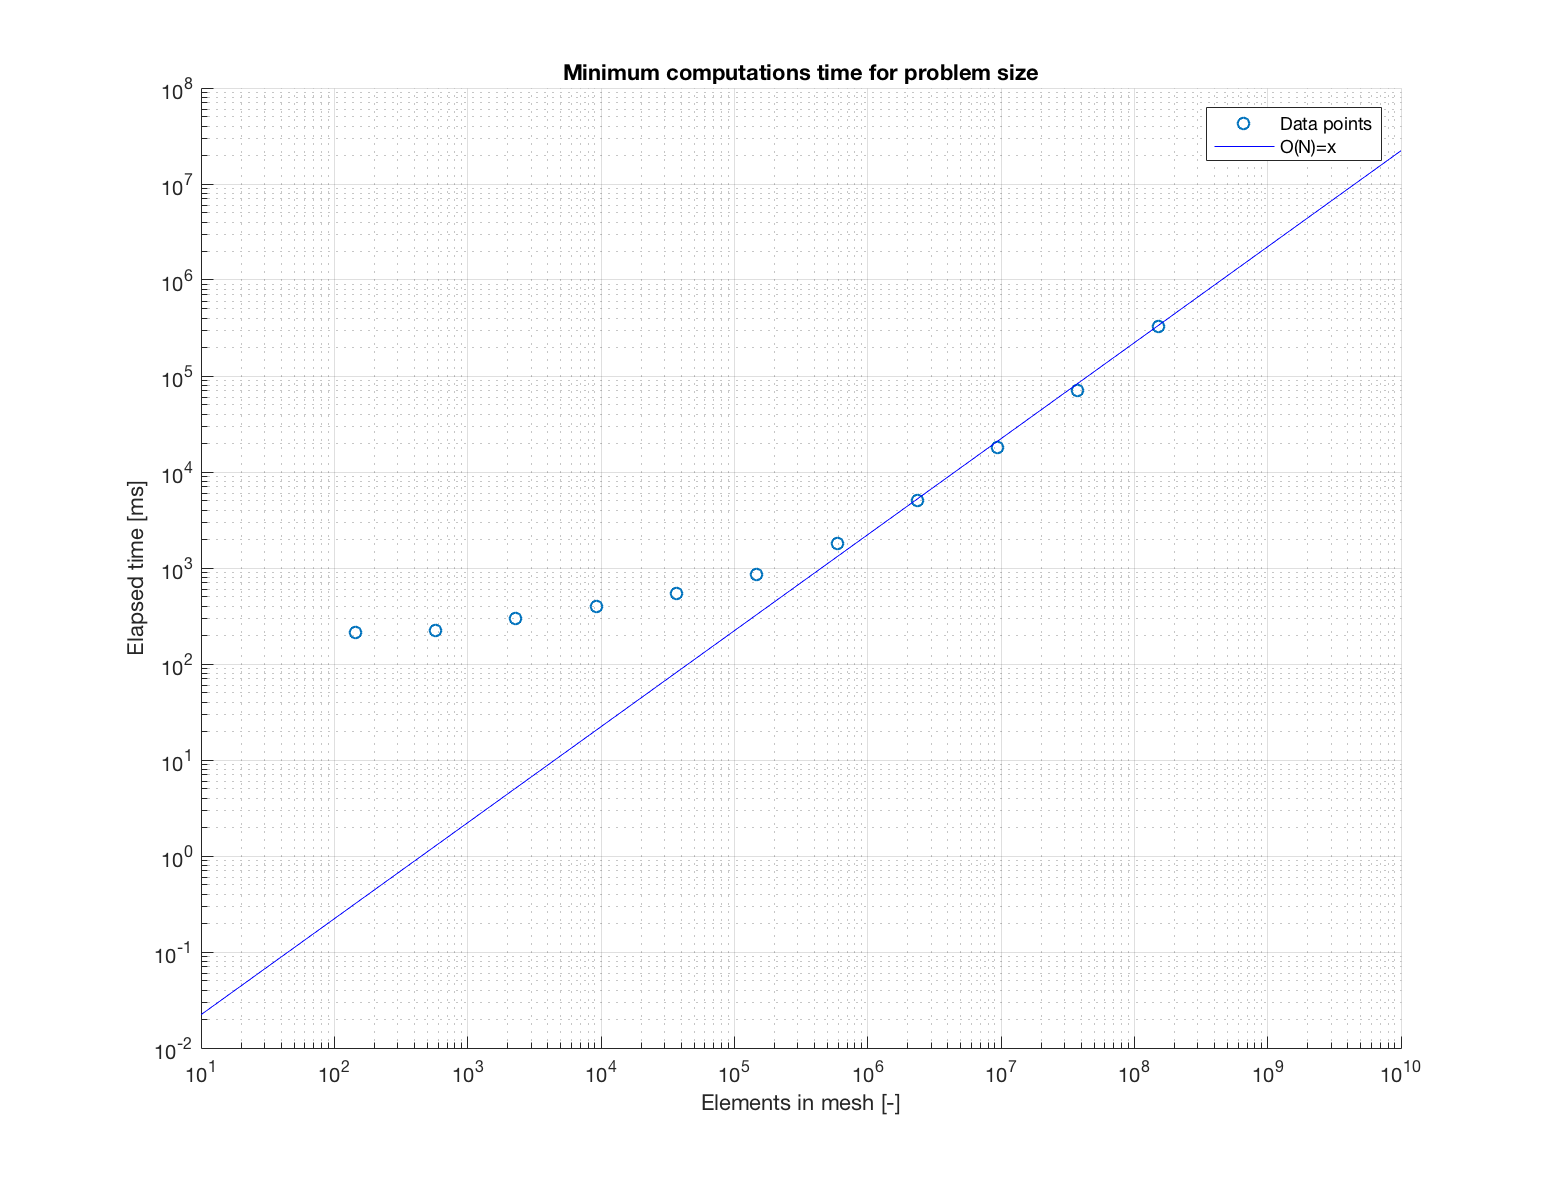
\includegraphics[width=0.9\textwidth]{img/upScalability.png}
    \end{figure}
    
    {\tiny * Run on a cluster of 6 machines - Westmere E56xx/L56xx/X56xx (Nehalem-C 2.7GHz) 4 CPU / 8GB RAM each}

\end{frame}

%%%%%%%%%%%%%%%%%%%%%%%%%%%

\begin{frame}{Implementation - scaling out}

\begin{figure}
      \centering
      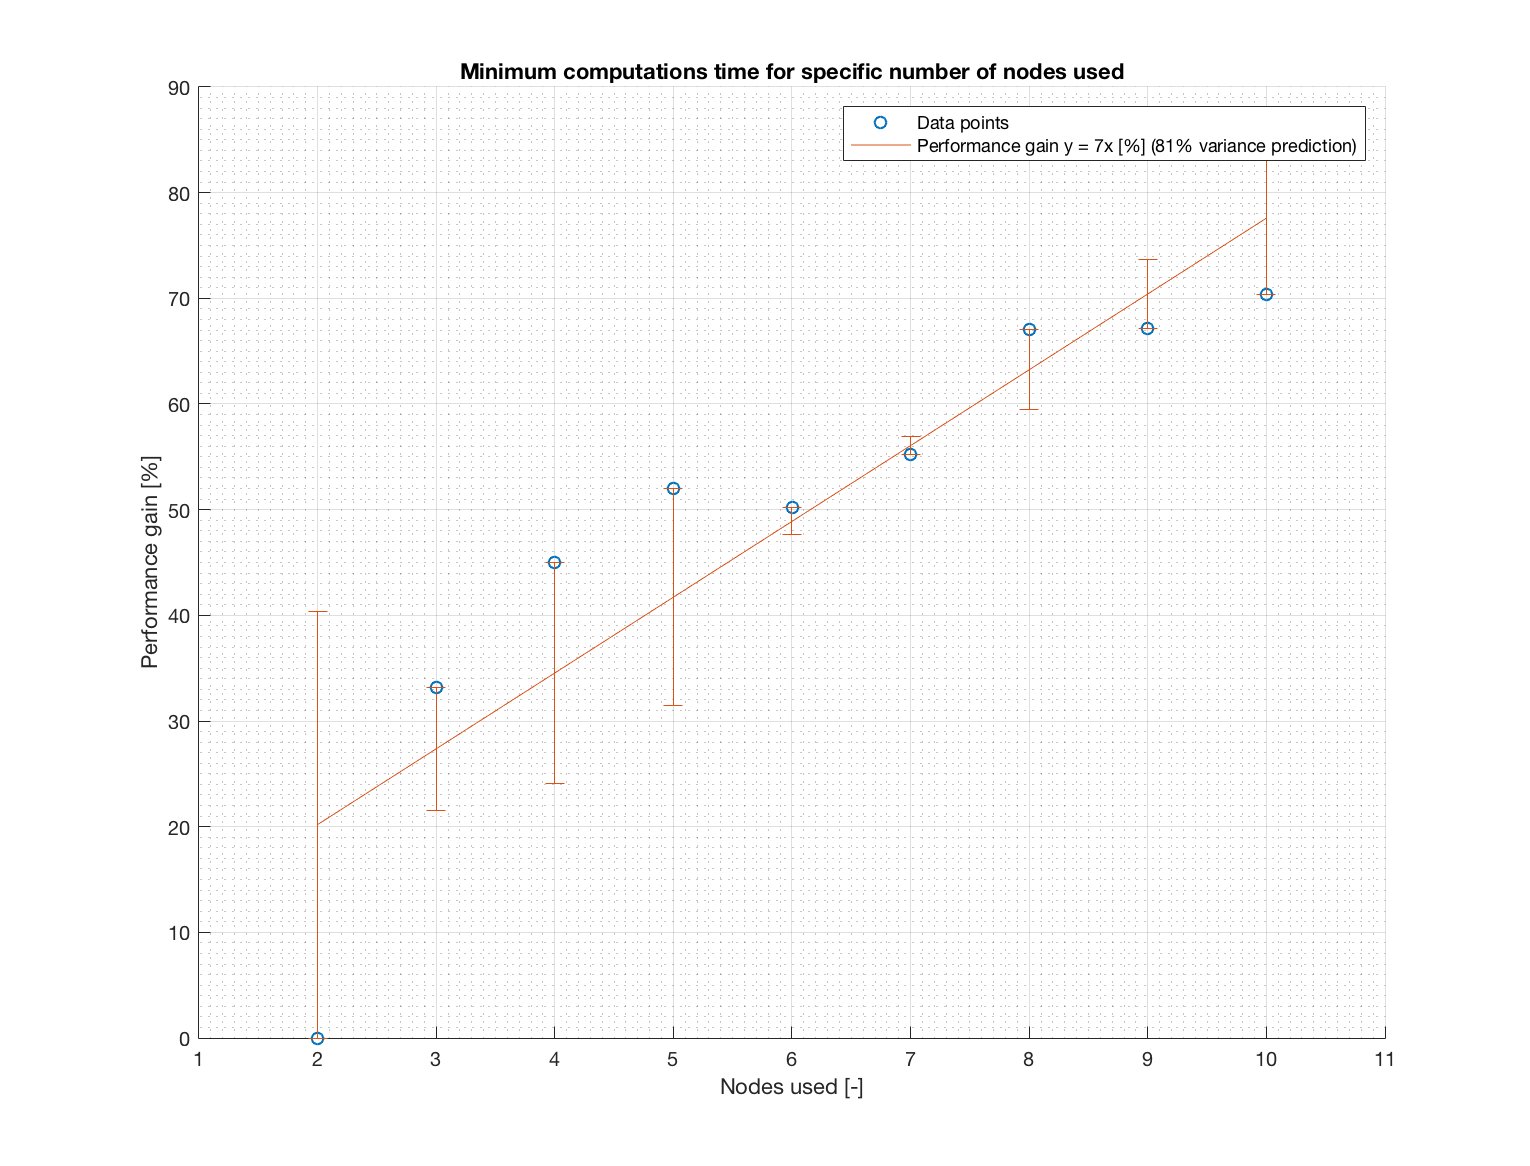
\includegraphics[width=0.9\textwidth]{img/outScalability.png}
    \end{figure}
    
    {\tiny * Run on the same cluster for an exemplary problem of heat transfer using 36 million elements. }

\end{frame}

%%%%%%%%%%%%%%%%%%%%%%%%%%%

\begin{frame}{Conclusions}

\begin{itemize}
  \item Distributed memory implementation is slower than shared memory one for small problem sizes which fit into physical memory of a single machine
  \item It can solve any problem by adding additional nodes (4 - 6144, 6 - 12288, 10 - 24576)
  \item Given there is a shared memory machine with sufficient physical memory, IMDG implementation outperforms it starting from a certain problem size
  \item This implementation can be made significantly faster by pushing some logic into worker nodes
\end{itemize}

\end{frame}
%%%%%%%%%%%%%%%%%%%%%%%%%%%

\begin{frame}{Thank you!}


Our research is funded by Polish National Science Centre \\ grant no. DEC-2015/19/B/ST8/01064

\end{frame}

%%%%%%%%%%%%%%%%%%%%%%%%%%%
%%%%%%%%%%%%%%%%%%%%%%%%%%%

\end{document}
